\documentclass{article}
\usepackage[utf8]{inputenc}
\usepackage[a4paper, total={6in, 8in}]{geometry}
\usepackage{graphicx}
\graphicspath{ {figures/}   }


\title{15-411: L5 Written Report}
\author{Manganese}
\date{November 23, 2015}

\begin{document}

\maketitle

\section{Introduction}

For L5, we chose to implement 4 optimizations: dead code elimination, constant folding and propagation, precoloring registers, and inlining. We apply these at three different optimization levels, which are -O0, -O1, and -O2. At -O0, we apply no optimizations at all, not even register allocation. At -O1, we apply register allocation. At -O2, we apply all of our optimizations. Finally, using the new --unsafe flag, we allow our compiler to bypass checking of memory safety for even faster compilation. With all optimizations and unsafe mode, our compiler reaches a performance score of 0.7661. Below is a comparison of runtimes between O0, O1, and O2 (in unsafe mode, since that's what counted in the end).

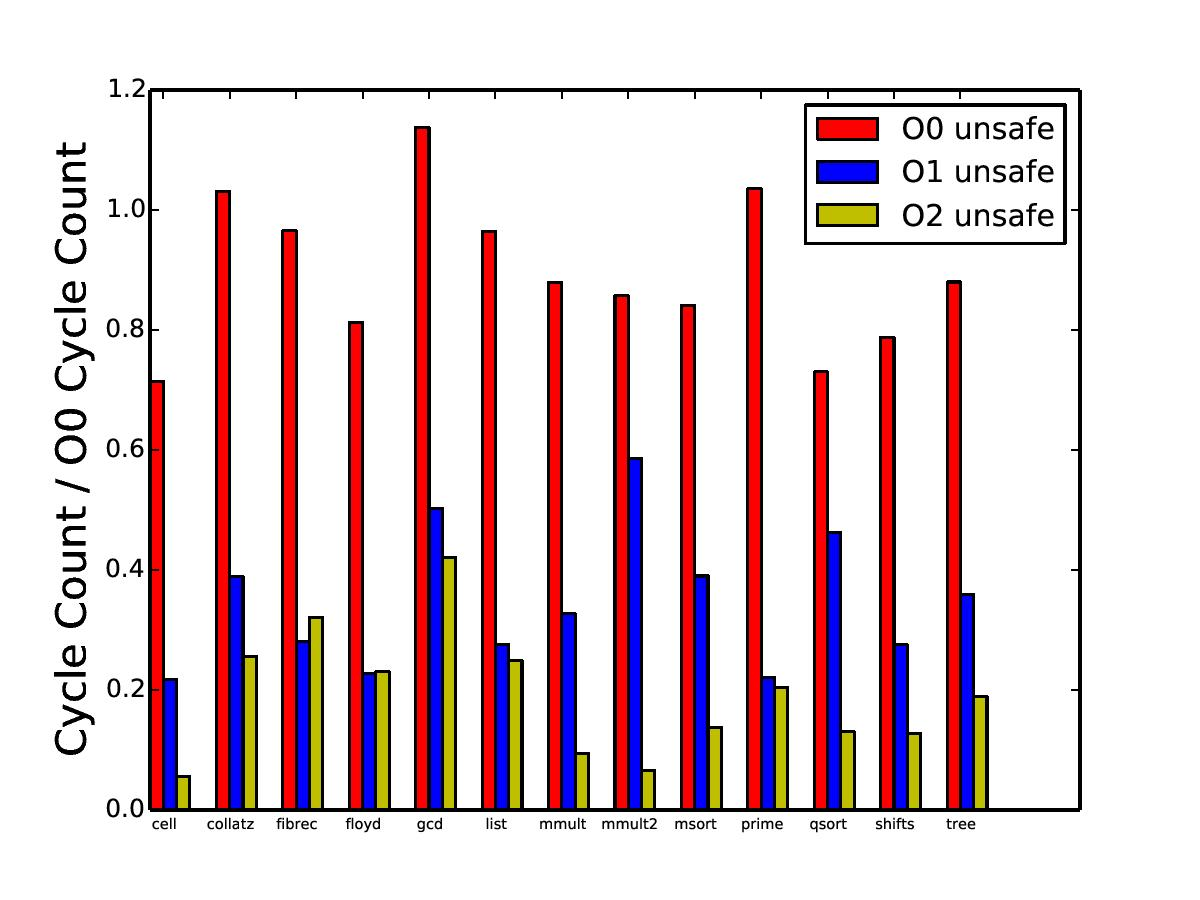
\includegraphics[scale=0.5]{O0-O1-O2_unsafe-page-001}

\section{Optimization 0: Unsafe Mode}

Unsafe mode allows us to assume that our compiler throws no exception. This means that we can forgo the checks for memory safety, such as making sure array accesses are in-bounds and there are no NULL pointer dereferences, as well as the number of bits for shifts. 

Below we include a graph that shows the effects of "--unsafe" in the compilation of the benchmark tests. As you can see, unsafe mode causes a large decrease in compilation time on most tests. 

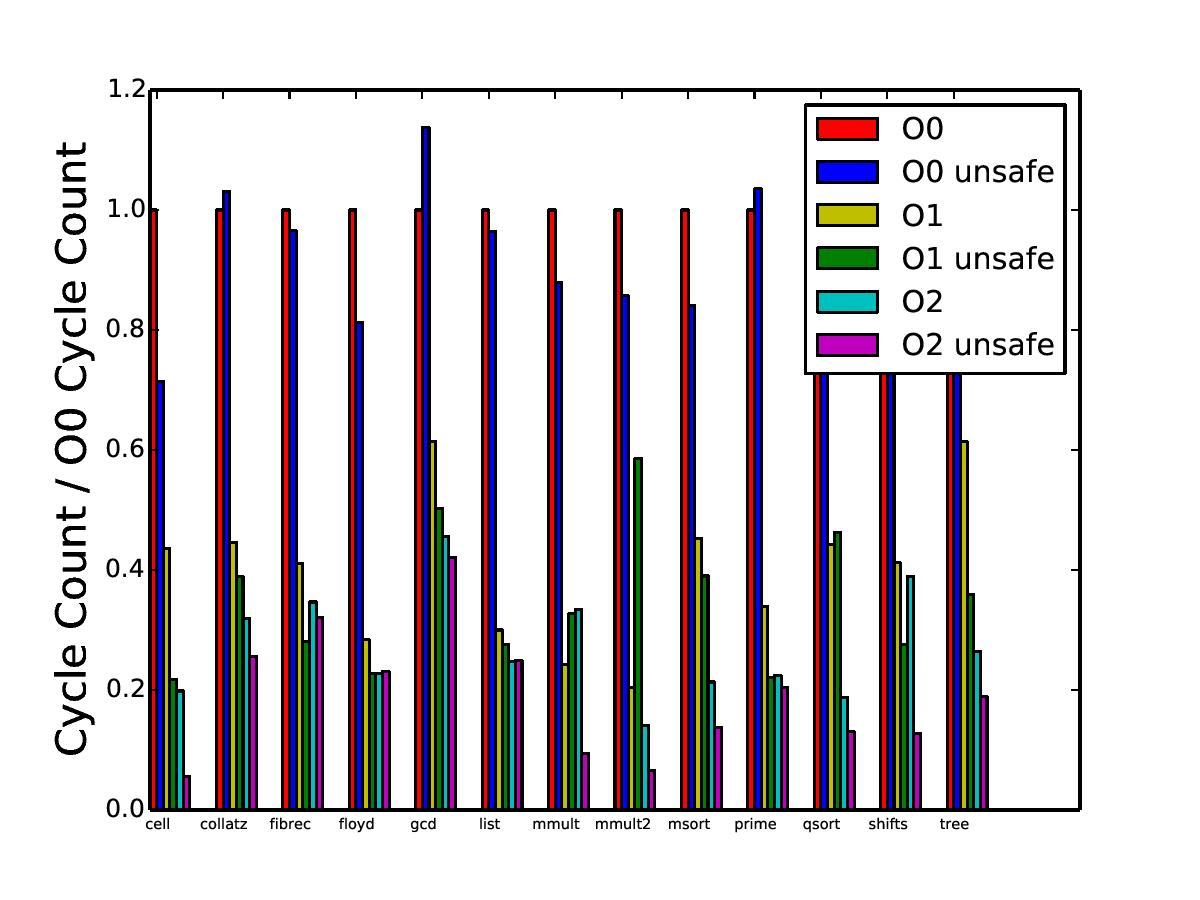
\includegraphics[scale=0.5]{everything-page-001}

Unsafe mode was (mostly) implemented in the conversion for the elaborated AST to what we called ``infinite-address code": sequential code with jumps, labels, cmps, but arbitrarily nested expressions, which is where we add the safety checks in safe mode.

\section{Optimization 1: Dead Code Elimination}

We eliminate dead code in each function as follows. First, we made a set of every single temp used in the function. We then map these temps to the lines that they're needed on using neededness rules 1 and 3 as described in lecture. This "seeds" the neededness for each temp. Then, using neededness rule 2, we propagate each temp's neededness in a backward dataflow analysis until we reach a line where the temp is already marked as needed or defined. 

On its own, dead code elimination improved only the performance of our compiler on the collatz, qsort, shifts, and tree tests. We do not know why this is, because these four tests do not seem to have one thing in common that other tests do not share. However, we hypothesize that in the tests this optimization did not help, the additional pass made to find and eliminate dead code was simply useless because few of the normal tests and none of the tests in the benchmark suite actually contained any dead code in the form of unused variables. It did help in eliminating some of the extraneous moves we generated, but that was only in combination with constant folding and propagation. Below we include a graph that shows the effects on performance with and without dead code elimination in isolation.

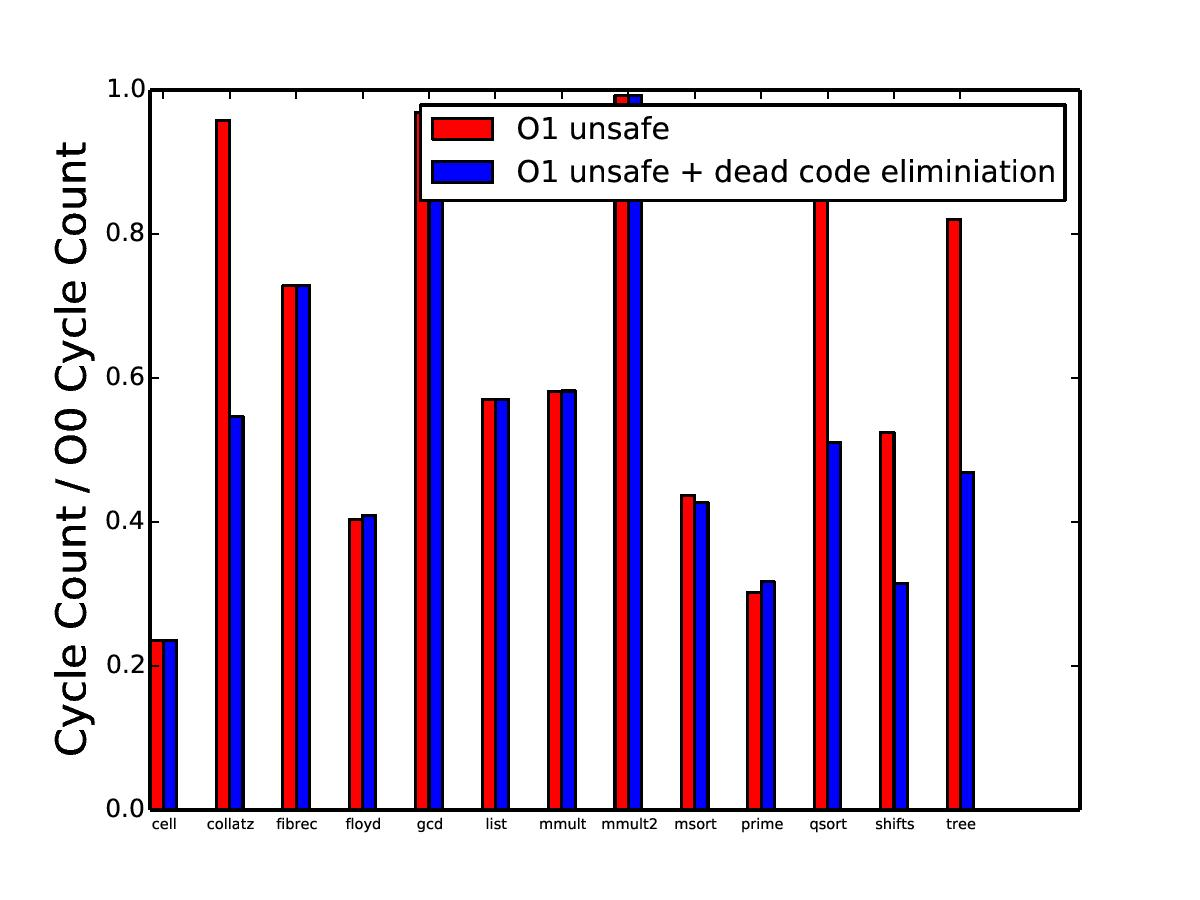
\includegraphics[scale=0.5]{O1_vs_deadcode-page-001}

Dead code elimination was performed on our two-address code.

\section{Optimization 2: Constant Folding and Propagation}

We implemented a weak form of constant folding and propagation due to not implementing SSA or reaching definitions. In order to avoid possibly propagating across jumps, we only propagate for temps defined exactly once in the program. Using a forward dataflow analysis, we find all temps, and if they are mapped to a constant in a move, replace all subsequent instances of this temp in the program with that constant. We then remove the move instruction. Finally, if we ever reach an instruction where after constant propagation we have a binop on two constant arguments, we simply fold them and map the temp to the new constant, creating another propagable temp.

On its own, constant folding and propagation did little to improve the performance of our compiler, and in tests mmult, msort, prime actually decreased performance by about 40, 30, and 20 percent respectively. While some of the slowdown can be explained by the additional pass made to find propagable temps, the rest can only be explained by "weird voodoo magic". On the tests where this optimization did help, we see a max increase in performance of about 30 percent. Without SSA form or reaching definitions, this optimization does not reach its full potential. It did help in eliminating some of the extraneous moves we generated, but that was only in combination with dead code elimination. Below we include a graph that shows the effects on performance with and without constant folding and propagation in isolation.

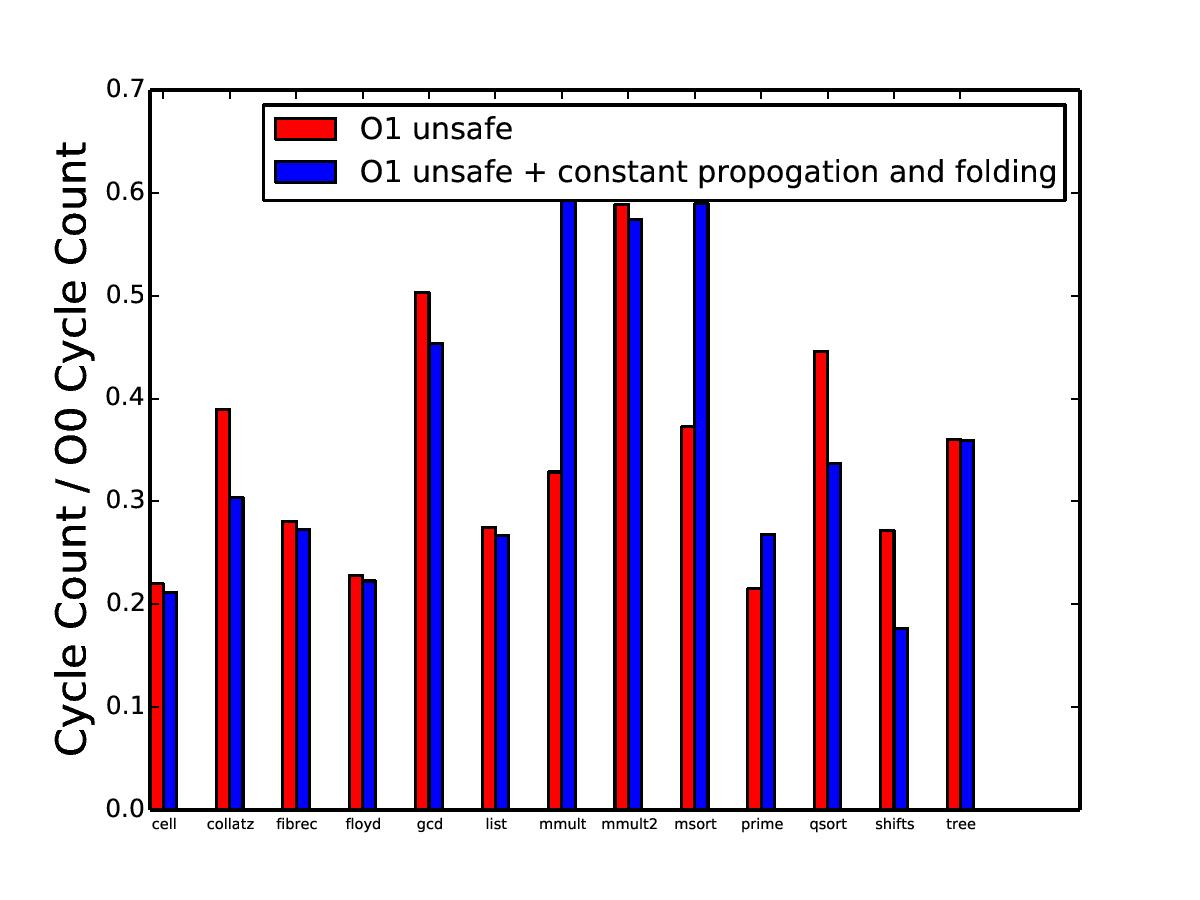
\includegraphics[scale=0.5]{O1_vs_constOpts-page-001}

Constant folding and propagation was performed on our three-address code.

\section{Optimization 3: Precoloring Temps}

The calling conventions specify six registers to be used for passing arguments to function. Up until L5, we reserved those registers for use only as arguments. After reserving two registers for handling memory-to-memory operations, using RBP as the base pointer, and reserving EAX to hold return values, this left us with only five registers to be allocated for arbitrary temps.

To handle this, we implemented the ability to precolor temps. This allowed us to require that certain temps be allocated certain registers, without losing the ability to allocate that register to other temps. This provided us with four more registers to allocate (we still reserved ECX and EDX for shifts and division, respectively). 

This turned out to be the most effective optimization we implemented. Unfortunately, the way we implemented precoloring made it difficult to toggle whether or not argument registers could be allocated elsewhere. To demonstrate the effect of having extra registers to allocate, we implemented a flag which sets how many of the original five general purpose registers to allocate (making the overall number of registers available to allocate at least four, and at most nine).

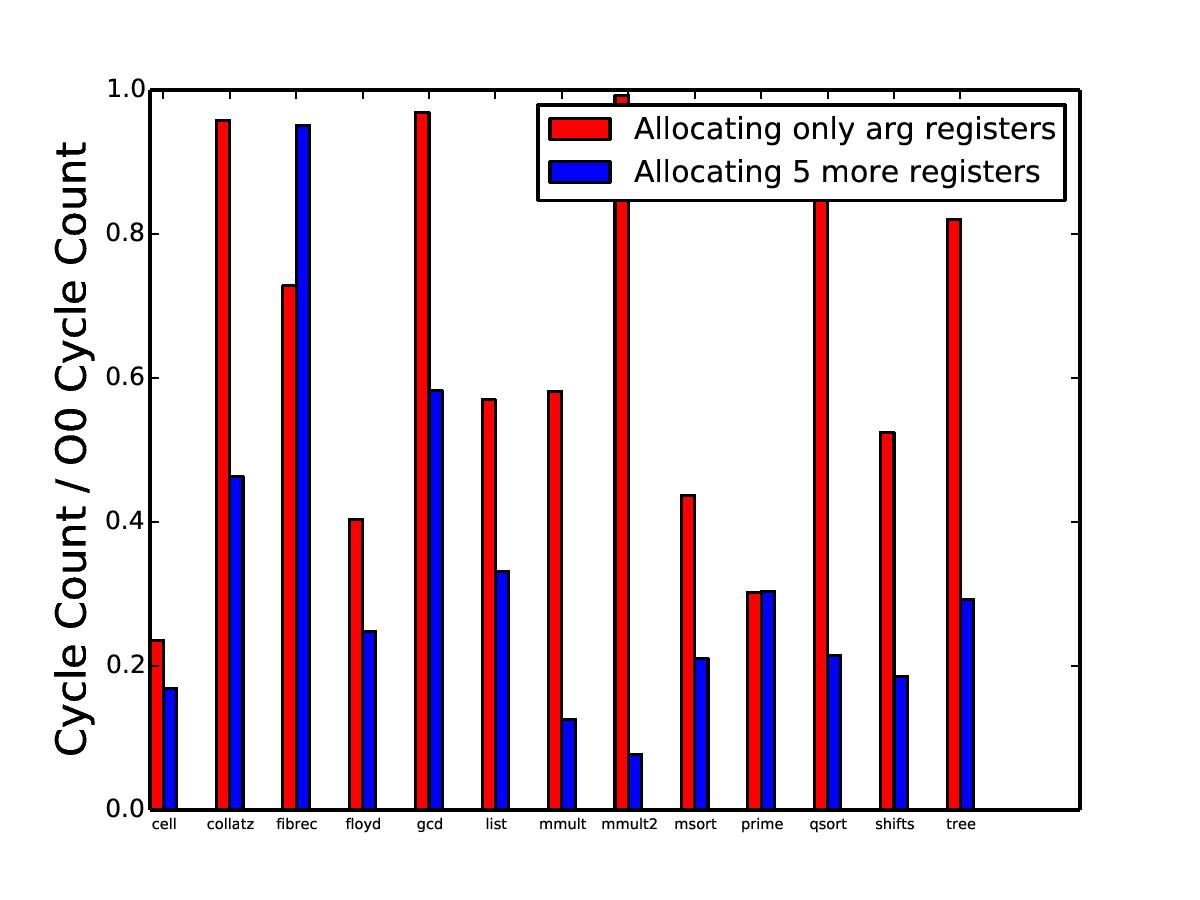
\includegraphics[scale=0.5]{allocating_more_regs-page-001}

As we can see, having additional registers to allocate drastically improves performance on almost all tests, with fibrec and prime being the only exceptions. One possible reason for this is that these two tests have very few temps that need to be allocated to registers, while being naive in their implementation (canonic inefficient implementations of fib and isPrime lead to a large number of redundant computations). 

\section{Optimization 4: Inlining}

We performed standard function inlining on our three-address code. The most effective heuristic we found was to inline a function if:

1. It was not recursive, including any level of mutual recursion, and
2. The function length was most 50 lines (in three-address code).

We also found it effective to ``recursively" inline functions. For example, suppose $f$ calls $g$ within a loop, but all $g$ does is call $h$ once. Then just inlining $g$ into $f$ will leave the $f$ with a call to $h$. It is more effective actually inline $h$ into $g$, and then inline the resulting code into $f$. We ended up inlining to a depth of 3, although we found little variation in performance at about a depth of 2.

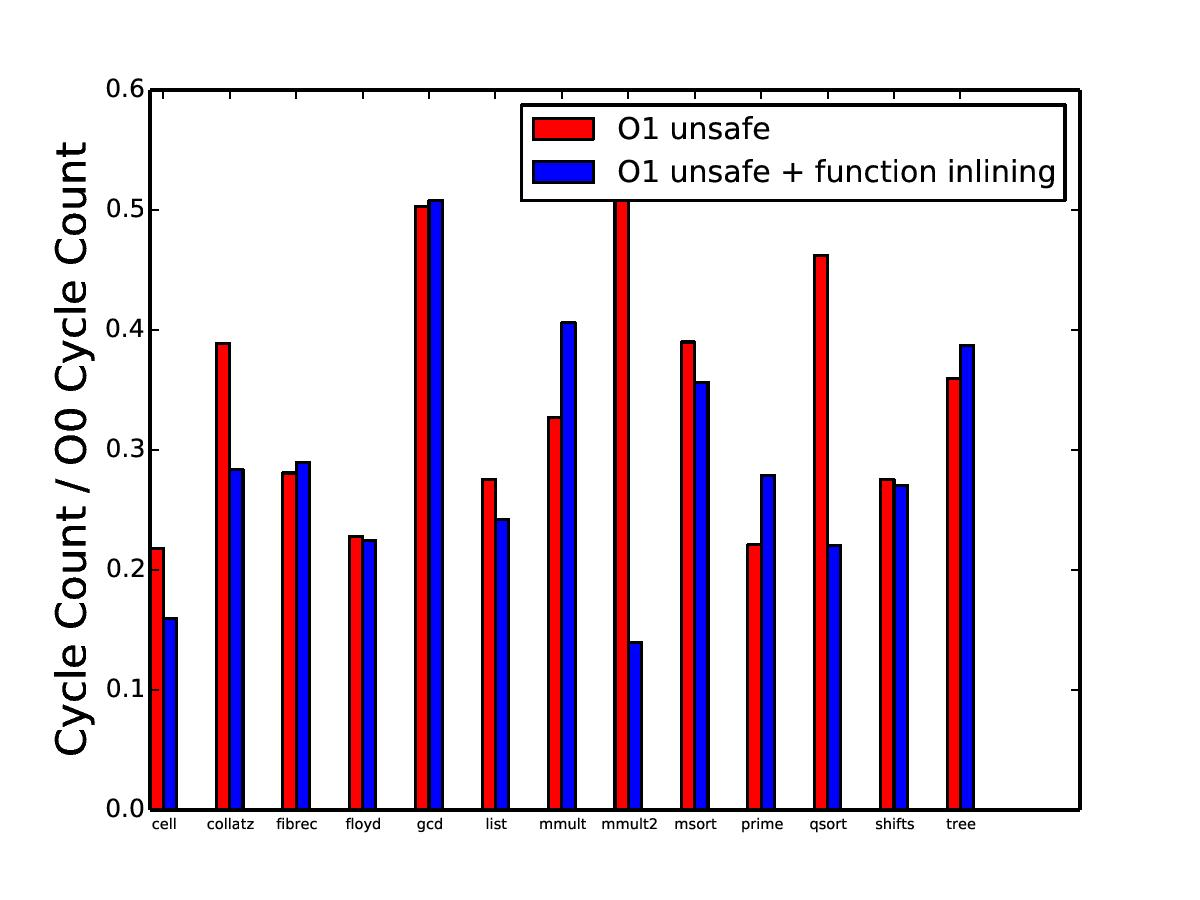
\includegraphics[scale=0.5]{O1_vs_inlining-page-001}

As we can see, inlining increased performance by a non-trivial amount in tests with many small functions calling each other, such as cell, qsort, and mmult2. In tests such as fibrec, floyd, and shifts, performance remained mostly the same because we either had recursive functions (which didn't get inlined) or not many functions calling each other (so inlining didn't really get used much). 

\section{Optimization 5: Limiting Push/Pop Instructions}

A final optimization involved the limiting of push/pop instructions relating to function calls. Previously, each function pushed/popped all of the registered it used both upon entrance, and before it made any function call. This let us avoid dealing with callee/caller conventions, but amounted to each function pushing/popping twice as much as necessary.

In L5, we changed register allocation so that each function pushes all of the registers it uses before it makes a function call, but only the main function pushes upon entrance. We effectively set up our own callee convention, where all registers are caller-saved.

However, we still have to deal with external functions which use a different calling convention. This is why main must push registers upon entrance as well: so as to not modify the contents of callee-saved registers. However, we never have to deal with this in any other case, since main is the only one of our functions that is called from an external function. This is why we chose to treat all registers are caller-saved instead of callee-saved (if we had done that, we would have had to deal with every case where we called an external function).

Although this did not significantly improve runtime across the board, it did drastically speed up collatz. This makes sense, since a recursive function with have many recursive calls, so the excessive pushing/popping for function calls had a greater cost.

This optimization also let us pass a few test cases in tests1 that we were stack overflowing on previously, so that was cool too.

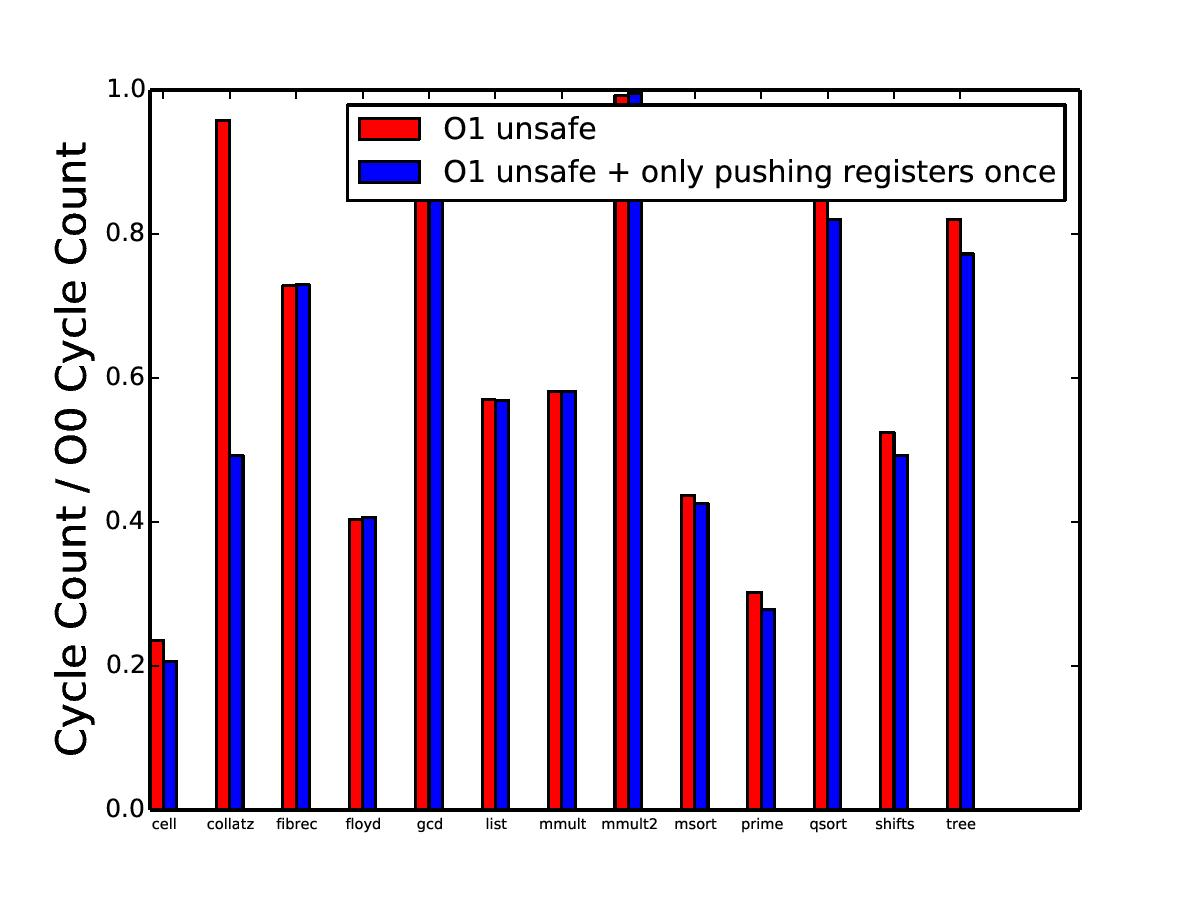
\includegraphics[scale=0.5]{O1_vs_onlyPushOnce-page-001}

\section{Weird Things}

In testing the efficacy of our optimizations, we saw that the best individual optimization was clearly the revamp made on the register allocator. Before the optimization, our compiler did not efficiently exploit registers. We pushed and popped every register in every function call, didn't allow use of registers reserved for specific operations, and spilled a ton of temps onto the stack. This resulted in reads to and writes from memory that could've been prevented by having more registers.

There are several occurrences of note in this lab. First, there were several points during the lab when we experienced some strange timing issues. At one point unsafe mode caused the results for the mmult benchmark to be slower by a factor of 3. At another, our optimizations were causing significant slow-downs in the execution of some tests, and significant speed-ups in others. We haven't been able to come up with a reason behind these occurrences besides what Rob calls "weird voodoo magic".

\end{document}



